%!TEX root = ../../thesis.tex

\section{A minimalist proof}
\label{chapter:limitations:proof}

It is of paramount importance to understand the properties of our algorithm, and to be able to have some certitude about its convergence and accuracy properties. The work presented in this thesis neglected this aspect and relied only on empirical evaluation. In the following of this section, we present a proof about the principle of our algorithm under restricted condition.

% The next step for a motivated person it to work on a formalism of our problem and to derive some useful proof about some properties of the algorithm.

\subsection{Problem and assumptions}

We consider a robot in a discrete state and action world. A teacher is providing feedback instructions to the robot through the use of a simple interface with two buttons, one button for ``correct'' and one button for ``incorrect''. But the mapping between the buttons and the meanings is unknown to the robot at start. This simplified setting allows studying specific details of the algorithm in more details, without the problem of dealing with continuous signals.

We assume that the user is coherent and uses one button for one meaning, and always the same button for the same meaning. Therefore, as exemplified in Figure~\ref{fig:proofmapping} the mapping between symbolic signals and their meaning can only be of two forms. 

\begin{figure}[!htbp]
\centering
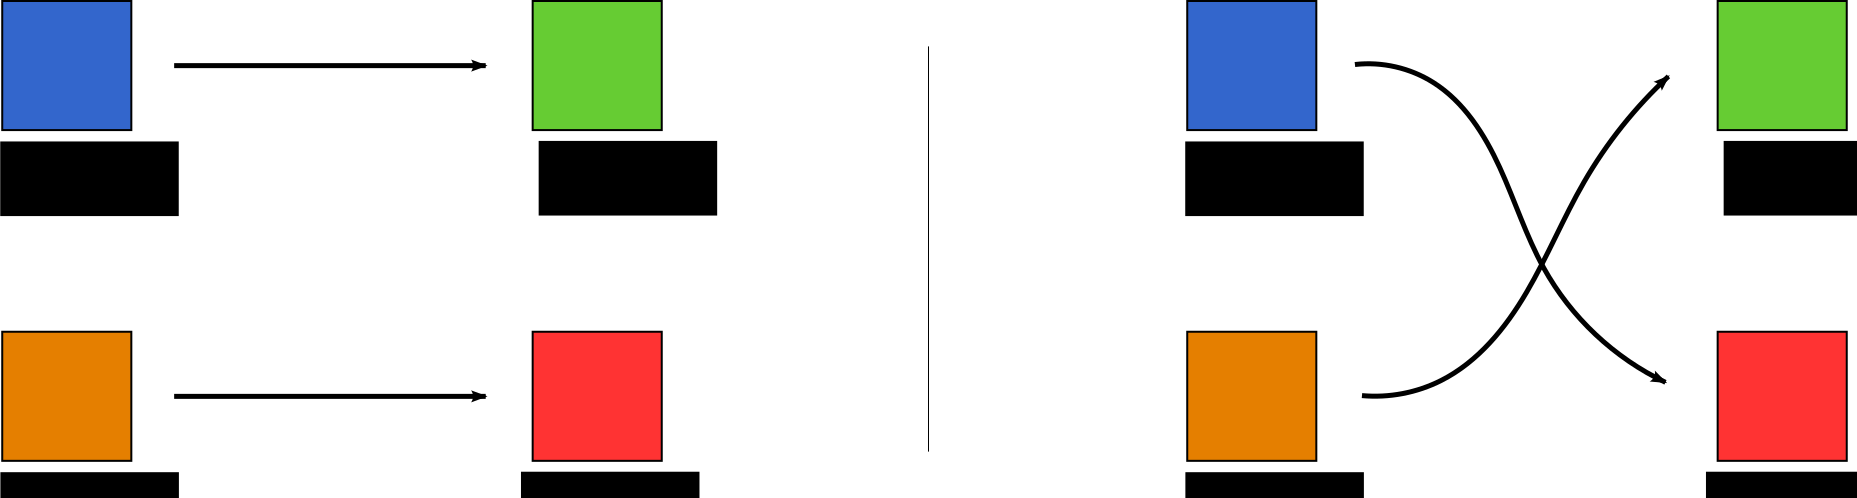
\includegraphics[width=\columnwidth]{\visualspdf/proof/mappings.pdf}
\caption{The two possible button to meaning mapping.}
\label{fig:proofmapping}
\end{figure} 

We further assume the robot is provided with a set of task hypothesis ($\xi_1,\ldots,\xi_T$), represented by their associated policies ($\pi_1, \ldots, \pi_T$). This set includes the task $\hat{\xi}$, the teacher as in mind, and when the robot performs an optimal action according to the optimal policy $\hat{\pi}$, the teacher presses the button associated to the ``correct'' meaning. He respectively presses the button associated to the ``incorrect'' meaning for a non-optimal action. We assumed that the teacher never makes teaching mistakes.

We define a number of terms that will simplify the notation in further subsections. $nS$ is the number of states in the environment, $nA$ is the number of actions available to the robot, and $nSA$ is the number of state-action pairs an agent can visit, which is simply $nS * nA$. We note as $diff(\pi_t, \pi_u)$ the number of optimal state-action pairs that differs between the optimal policies $\pi_t$ and $\pi_u$ respectively associated to the task $\xi_t$ and $\xi_u$. Therefore the ratio of optimal state-action pairs that differs between two task hypothesis is denoted as $\frac{diff(\pi_t, \pi_u)}{nSA}$. 

The $diff()$ function logically outputs $0$ when comparing one task to itself, i.e. $diff(\pi_t, \pi_t) = 0$. And a ratio of 1 means the two tasks are symmetric (see discussion about symmetry in section~\ref{chapter:lfui:symmetries}), which means whatever the action the robot will choose, the meaning inferred according to the first task will be the opposite of the meaning inferred according to the second task. This property, as will be seen in our minimalist proof, does not allow differentiating between two symmetric tasks.

\subsection{Illustration}

Before describing our simple proof, it is important to have an intuition on the relation between the buttons and the meanings in different conditions. We consider again our T world scenario as an illustration (see chapter~\ref{chapter:lfui:example}).

Figure~\ref{fig:proofsymbolic} shows all possible button presses sequences expected from the teacher in different conditions. On top are the state-action pairs considered (a). (b) and (c) lines represent the expected meanings for each of the state-action pairs and according to the hypothesis G1 (b) or G2 (c). (d) and (e) lines represent the possible button presses sequence of the teacher when teaching hypothesis G1 and considering the two possible mappings. Respectively (f) and (g) for hypothesis G2.

\begin{figure}[!htbp]
\centering
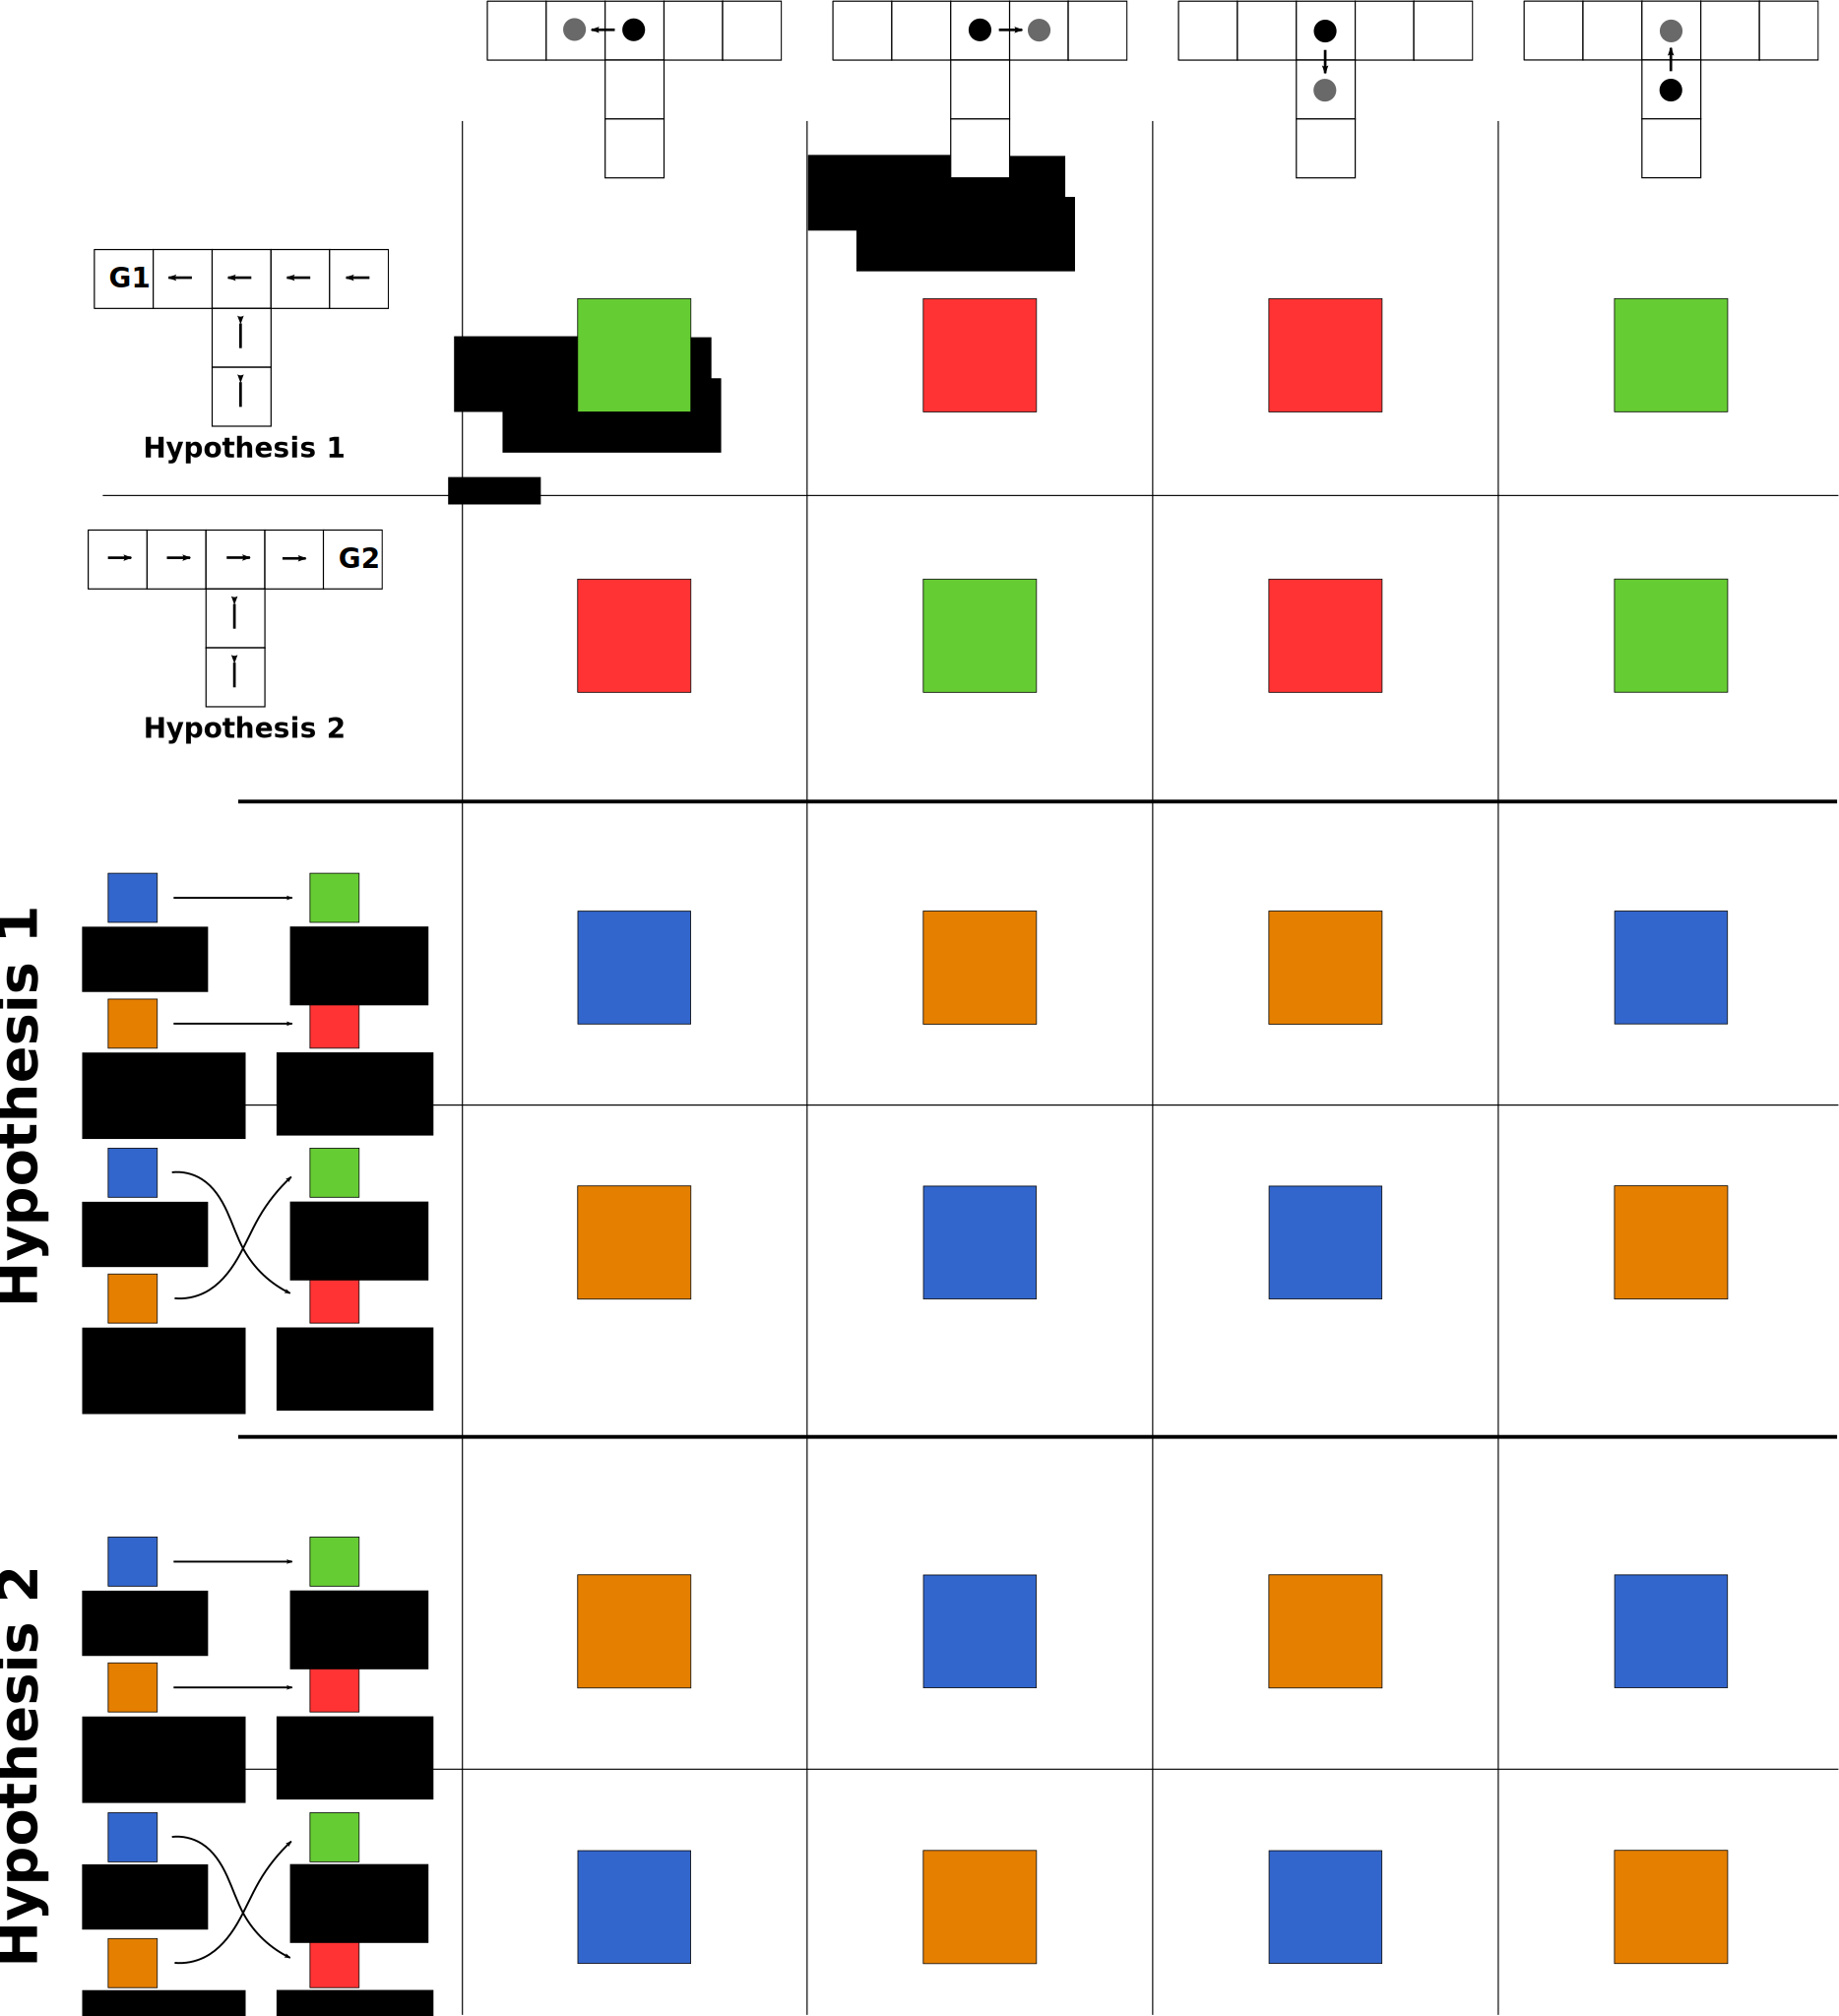
\includegraphics[width=\columnwidth]{\visualspdf/proof/symbolic_feedback.pdf}
\caption{Illustration of the teacher's button presses for several state-action pairs. On top are the state-action pair considered (a). (b) and (c) lines represent the expected meanings for each of the state-action pairs and according to the hypothesis G1 (b) or G2 (c). (d) and (e) lines represent the possible button presses sequence of the teacher when teaching hypothesis G1 and considering the two possible mappings. Respectively (f) and (g) for hypothesis G2.}
\label{fig:proofsymbolic}
\end{figure} 

First, before entering into more detail, given the extensive number of assumptions defined, for the simple example of Figure~\ref{fig:proofsymbolic} it would be easy to find the correct hypothesis by visiting only two state-action pairs. Indeed as taking an action in the trunk of the T will be interpreted similarly by both hypotheses, and given the user is not making teaching mistakes and is coherent in its use of the buttons, we could instantaneously know the meaning of the button pressed and therefore the meaning of the other button. Then taking an action in the top bar of the T would allow us to differentiate between G1 and G2. However we will not exploit this type of properties for our proof and we remind that in all the experimental scenarios presented in this thesis, there were no state-action pairs that allowed for an unequivocal interpretation of a signal.

For the purpose of our demonstration, we should read this figure by comparing lines (d), (e), (f), and (g) with the expectation from lines (b) and (c). We will denote $B$ the blue button, $O$ the orange button, $C$ the ``correct'' meaning (the green patch), and $W$ the ``incorrect'' meaning (the red patch, $W$ for wrong). For example, let's imagine we receive the sequence of presses of line (d) that we note $[B,O,O,B]$. For hypothesis 1 (G1) we expected $[C,W,W,C]$, and for hypothesis 2 (G2) we expected $[W,C,W,C]$. 

Given these two possible interpretations we can build a statistical model for the signal to meaning mapping. For G1, we obtain the following model $p(C|B, G1) = \frac{2}{2} = 1$, $p(C|O, G1) = \frac{0}{2} = 0$, and $p(W|B, G1) = \frac{0}{2} = 0$, $p(W|O, G1) = \frac{2}{2} = 1$. To simplify notation we note $[1,0]_{B,G1}$ and $[1,0]_{O,G1}$ the model for each button where the first element of the vector is the probability associated to the ``correct'' meaning and the second is the one associated to the ``incorrect'' meaning. And the underscript details the button and the task considered. Using the same reasoning, again for line (d) but for hypothesis G2, the classifier is: $[0.5,0.5]_{B,G2}$ and $[0.5,0.5]_{O,G2}$.

In this thesis, as we were not considering symbolic signals, and used a metric that compares the expectation from the frame (i.e. lines (b) and (c)) with prediction from the classifier associated to each task. Let's use Equation~\ref{eq:matchingoverfitting} to compute the likelihood for each task. We remind the likelihood equation:
%
\begin{eqnarray}
\L(\xi_t) &=& \prod_{i = 1,\ldots,M} p(l^c_i = l^f_i | D_M, \xi_t) \nonumber \\ 
&=& \prod_{i = 1,\ldots,M} \sum_{k = 1, \ldots, L} p(l^c_i = l_k | e_i, \theta_M) p(l^f_i = l_k | s_i, a_i, \xi_t) \nonumber
\end{eqnarray}
%
where $p(l^c_i = l_k | e_i, \theta_M)$ is the classification of the signal $e_i$ from our classification model $\theta_M$, and $p(l^f_i = l_k | s_i, a_i, \xi_t)$ is the expected label given by the frame.

For G1 we obtain:
%
\begin{eqnarray}
\L(G1) &=& \left((1\times1)+(0\times0)\right)\left((0\times0)+(1\times1)\right)\left((0\times0)+(1\times1)\right)~\ldots  \nonumber \\
&& \ldots~\left((1\times1)+(0\times0)\right)  \nonumber \\
&=& 1 \nonumber
\end{eqnarray}

And for G2 we obtain:
%
\begin{eqnarray}
\L(G2) &=& \left((0.5\times0)+(0.5\times1)\right)\left((0.5\times1)+(0.5\times0)\right)~\ldots  \nonumber \\
&& \ldots~\left((0.5\times0)+(0.5\times1)\right)\left((0.5\times1)+(0.5\times0)\right) \nonumber \\
&=& 0.0625 \nonumber
\end{eqnarray}

By normalizing the likelihoods, we obtain the probability of each task: $p(G1) \approx 0.94$ and $p(G2) \approx 0.06$. We see that our measure of likelihood is able to identify the correct task. The same process can be repeated for each case (i.e. (e), (f), and (g)) and will always identify the correct hypothesis.

Given this explanation, we can start drafting the proof, but, to simplify further the proof, we will add an additional assumption.

\subsection{The proof}

In order to make the proof simple and illustrative, we assume each hypothetic policy has an equal number of optimal state-action pairs than of non-optimal state-action pairs. Therefore when the agent has visited once all the state-action pairs, it has collected the same amount of signals with label ``correct'' than with label ``incorrect''. It ensures that, when the agent has visited once all the state-action pairs, the user will have pressed as many time the blue button than the orange button, exactly $\frac{nSA}{2}$ times. But it also ensures that all interpretation hypotheses estimated that half of the labels are of meaning ``correct'' and half are of meaning ``incorrect''. Therefore, if the agent visits once all the state-action pairs, the signal to meaning model for each class (i.e. for $C$ and $W$) will be symmetric for every task hypothesis considered. 

% We can explain this effect as follows. First, for all hypothesis this assumption ensure that, when the agent has visited once all the state-action pairs, the user will have pressed as many time the blue button than the orange button, exactly $\frac{nSA}{2}$ times. And the same assumption ensures that whatever the task considered the number of ``correct'' and ``incorrect'' labels will be the same. However the number of blue button presses associated to ``correct'' or ``incorrect'' labels remains undefined and depends on the overlap between the true unknown policy taught by the teacher and the one considered by the agent in the labeling process. 

Therefore, we can evaluate the possible signal to meaning mappings based on the difference in policies between the optimal task and any hypothetic task using the $diff()$ function defined earlier. For a given task $\xi_t$ we can compute the ratio of optimal state-action pairs that are the same as for the true task $\hat{\xi}$, which we denote $\Upsilon_{\xi_t} = \frac{nSA - diff(\pi_t, \hat{\pi})}{nSA}$. The agent will never have access to this information and we only use this measure for our proof.

Given our previously defined assumption, and assuming the agent visited all state-action pairs once, if the user uses the blue ($B$) button to mean ``correct'', then the blue signal model will be $[\Upsilon_{\xi_t},1-\Upsilon_{\xi_t}]_{B,\xi_t}$. Which implies the orange button mapping is $[1-\Upsilon_{\xi_t},\Upsilon_{\xi_t}]_{O,\xi_t}$. Respectively, if the user uses the blue button to mean ``incorrect'', then the blue signal model will be $[1-\Upsilon_{\xi_t},\Upsilon_{\xi_t}]_{B,\xi_t}$. Which implies the orange button mapping is $[\Upsilon_{\xi_t},1-\Upsilon_{\xi_t}]_{O,\xi_t}$.

\subsubsection*{Deriving the likelihood with respect to $\Upsilon_{\xi_t}$}

Using this notation, we can write the likelihood equation as a product of vector's products. Where for example, $\sum_{k = 1, \ldots, L} p(l^c_i = l_k | e_i, \theta_M) p(l^f_i = l_k | s_i, a_i, \xi_t)$ can be written as $[\Upsilon_{\xi_t},1-\Upsilon_{\xi_t}]_{B,\xi_t}.[1,0]_{s_i,a_i,\xi_t}^T$ for those cases where the user pressed the blue button (i.e. $e_i = B$) after an optimal state-action pair (i.e. the expected meanings is ``correct'', i.e. $[1,0]_{s_i,a_i,\xi_t}$), and given that the blue button was the one used by the teacher to mean ``correct'', resulting in $[\Upsilon_{\xi_t},1-\Upsilon_{\xi_t}]_{B,\xi_t}$ as the button to meaning model.

We can now list all the possible cases. We can split the state-action pairs in half, the one that are optimal according to the teacher intended task $\hat{\xi}$ (there is $\frac{nSA}{2}$ of them) and the one that are non-optimal according to the teacher intended task $\hat{\xi}$ (there is $\frac{nSA}{2}$ of them). For the state-action pairs that are optimal, the user will press the button he uses to mean ``correct'' (i.e. the blue or the orange one), respectively for the non-optimal, he will press the other button (i.e. the orange or the blue one).

But the agent evaluates those button presses with respect to the task hypothesis currently considered $\xi_t$, which might not be the one the teacher as in mind. Therefore, only a fraction of the time the button presses match with what is expected by the task considered $\xi_t$. This number can be exactly identified as $\frac{nSA}{2}.\Upsilon_{\xi_t}$. Therefore for $\frac{nSA}{2}.\Upsilon_{\xi_t}$ state-action pairs, the ``correct'' button was pressed for the ``correct'' meaning. For one state-action pair, this represent an update of the likelihood function by $[\Upsilon_{\xi_t},1-\Upsilon_{\xi_t}].[1,0]^T$, which is simply $\Upsilon_{\xi_t}$. As there is $\frac{nSA}{2}.\Upsilon_{\xi_t}$ similar situations the update is $\Upsilon_{\xi_t}^{\frac{nSA}{2}.\Upsilon_{\xi_t}}$.

Similarly there is $\frac{nSA}{2}.(1-\Upsilon_{\xi_t})$, where the ``incorrect'' button was pressed for the ``correct'' meaning. Which represents an update of $[\Upsilon_{\xi_t},1-\Upsilon_{\xi_t}].[0,1]^T$, which is simply $1-\Upsilon_{\xi_t}$. As there is $\frac{nSA}{2}.(1-\Upsilon_{\xi_t})$ similar situations the update is $(1-\Upsilon_{\xi_t})^{\frac{nSA}{2}.(1-\Upsilon_{\xi_t})}$.

And, as the situation is symmetric for the non-optimal state-action pairs of the teacher intended task $\hat{\xi}$, the likelihood equation can be rewritten as:

\begin{eqnarray}
\L(\xi_t) &=& \Upsilon_{\xi_t}^{\frac{nSA}{2}.\Upsilon_{\xi_t}} \times (1-\Upsilon_{\xi_t})^{\frac{nSA}{2}.(1-\Upsilon_{\xi_t})} \times \Upsilon_{\xi_t}^{\frac{nSA}{2}.\Upsilon_{\xi_t}} \times (1-\Upsilon_{\xi_t})^{\frac{nSA}{2}.(1-\Upsilon_{\xi_t})} \nonumber \\
&=& \Upsilon_{\xi_t}^{nSA.\Upsilon_{\xi_t}} \times (1-\Upsilon_{\xi_t})^{nSA.(1-\Upsilon_{\xi_t})}
\label{eq:likelihoodproof} 
\end{eqnarray}

% Note that this equation is the same whatever the button chosen by the user to mean ``correct''.

% As there is the same number of ``correct'' and ``incorrect'' expected labels, we can factorize the likelihood equation as follows (see appendix~\ref{appendix:proof}):
% %
% \begin{eqnarray}
% \L(\xi_t) &=& \Upsilon_{\xi_t}^{nSA.\Upsilon_{\xi_t}} \times (1-\Upsilon_{\xi_t})^{nSA.(1-\Upsilon_{\xi_t})}
% \label{eq:likelihoodproof}
% \end{eqnarray}

Note that this equation is the same whatever the button chosen by the user to mean ``correct''. We can check our previous likelihood estimate in our simple example of Figure~\ref{fig:proofsymbolic} considering the 4 state-action pairs visited are the only one available in the world, and considering we receive button presses as in line (d). We obtain the same likelihoods as the one derived in the first subsection, i.e. $\L(G1) = 1^{1\times4} \times 0^{0\times4} = 1$ and $\L(G1) = 0.5^{0.5\times4} \times 0.5^{0.5\times4} = 0.5^4 = 0.0625$.

\subsubsection*{Analyzing the likelihood function}

We can plot the likelihood function with respect to the full range of value that $\Upsilon_{\xi_t}$ can take, i.e. between 0 and 1. We consider that $nSA = 1$ for now. Obviously such a value of $nSA$ is impossible in practice given our assumptions, we need as many optimal and non-optimal state-action pair, which means that $nSA$ must be an even number. However, now that we have our theoretical estimate of the likelihood function we shall study its properties in a theoretical way. Additionally, our equation is only valid if the agent visited all state-action pairs but for the sake of our analysis, we consider that the value of $nSA$ represents the number of state-action pair visited by the agent. Moreover, there exist a relation between the number of state-action pairs and the discrete set of value that $\Upsilon_{\xi_t}$ can take given our assumptions, but for the sake of the analysis we consider the full range of value between 0 and 1.

Figure~\ref{fig:prooflikelihoodone} shows the likelihood function for $nSA = 1$. As expected the likelihood value is higher for the correct task, i.e. when $\Upsilon_{\xi_t} = 1$, and decrease as the number of state-action pairs that differ increases, i.e. when $\Upsilon_{\xi_t}$ decrease. However this function holds an interesting property, which is that once more than half of the optimal state-action pair differs with the true task, the function increases again. Until is reaches a point where none of the optimal state-action pairs of the task are the same as for the true task. This specific case is what we called a symmetric task hypothesis, where the symmetric interpretation of the feedback signals is as likely as the correct interpretation of the signals. Indeed none of the state-action pairs allow breaking this symmetry for the feedback frame. 

Therefore, given all the assumptions considered, if the agent is provided with a set of task hypothesis, that included the correct task $\hat{\xi}$ but does not include any symmetric hypothesis (which means all tasks hold the following property $\Upsilon_{\xi_t} > 0$), we can guarantee that if the teacher visits all state-action pairs once, the user intended task $\hat{\xi}$ (which hold the property $\Upsilon_{\xi_t} = 1$) will have the greater likelihood. In other words: $\L(\hat{\xi}) > \L(\xi_t)$ if $\Upsilon_{\xi_t} \in~]0,1[$.

\begin{figure}[!htbp]
\centering
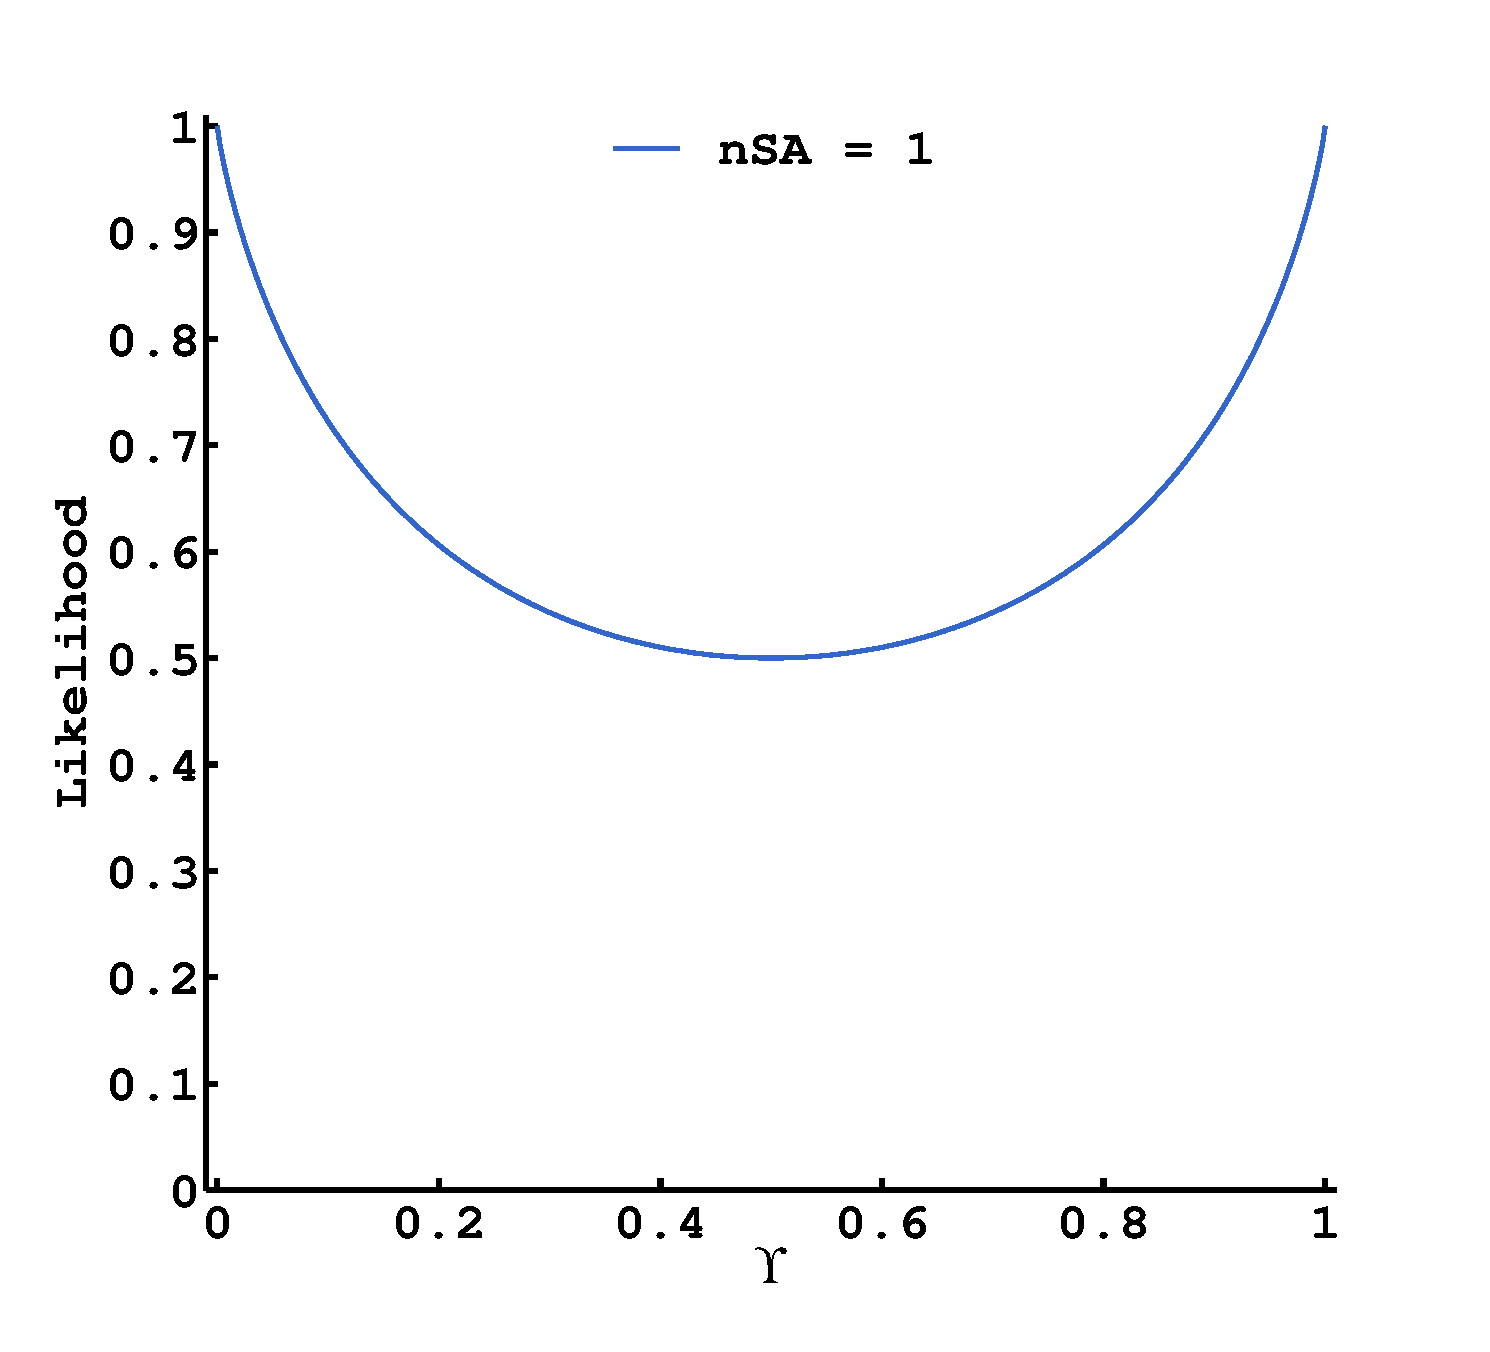
\includegraphics[width=\plotsize\columnwidth]{\imgpath/proof/likelihoodOne}
\caption{The likelihood function of Equation~\ref{eq:likelihoodproof} for $nSA =1$.}
\label{fig:prooflikelihoodone}
\end{figure}

\subsubsection*{Building confidence}

We now discuss the problem of estimating the confidence that one task is a better candidate than another one. Of course, in this setting, given the strong assumption that the user is never making mistakes, such confidence mechanism is not needed. However, we have seen in previous chapter that deciding when to stop is a critical part of the algorithm. The simplest method consists of normalizing the likelihood for each task defining a probability threshold above which a task is considered as the correct one. If we consider for example 10 task hypothesis with different values of $\Upsilon$, normalizing the likelihood when $nSA = 1$ won't produce a very sharp probability distribution on task. All tasks will roughly share the same probability. However, when visiting more and more states, the likelihood function becomes more and more sharp and only normalizing likelihoods will split the hypothesis apart. In the limit, when $nSA \rightarrow +Inf$, only the hypothesis with a better value of $\Upsilon$ (i.e. closer to 0 or 1) will reach a probability of 1.

\begin{figure}[!htbp]
\centering
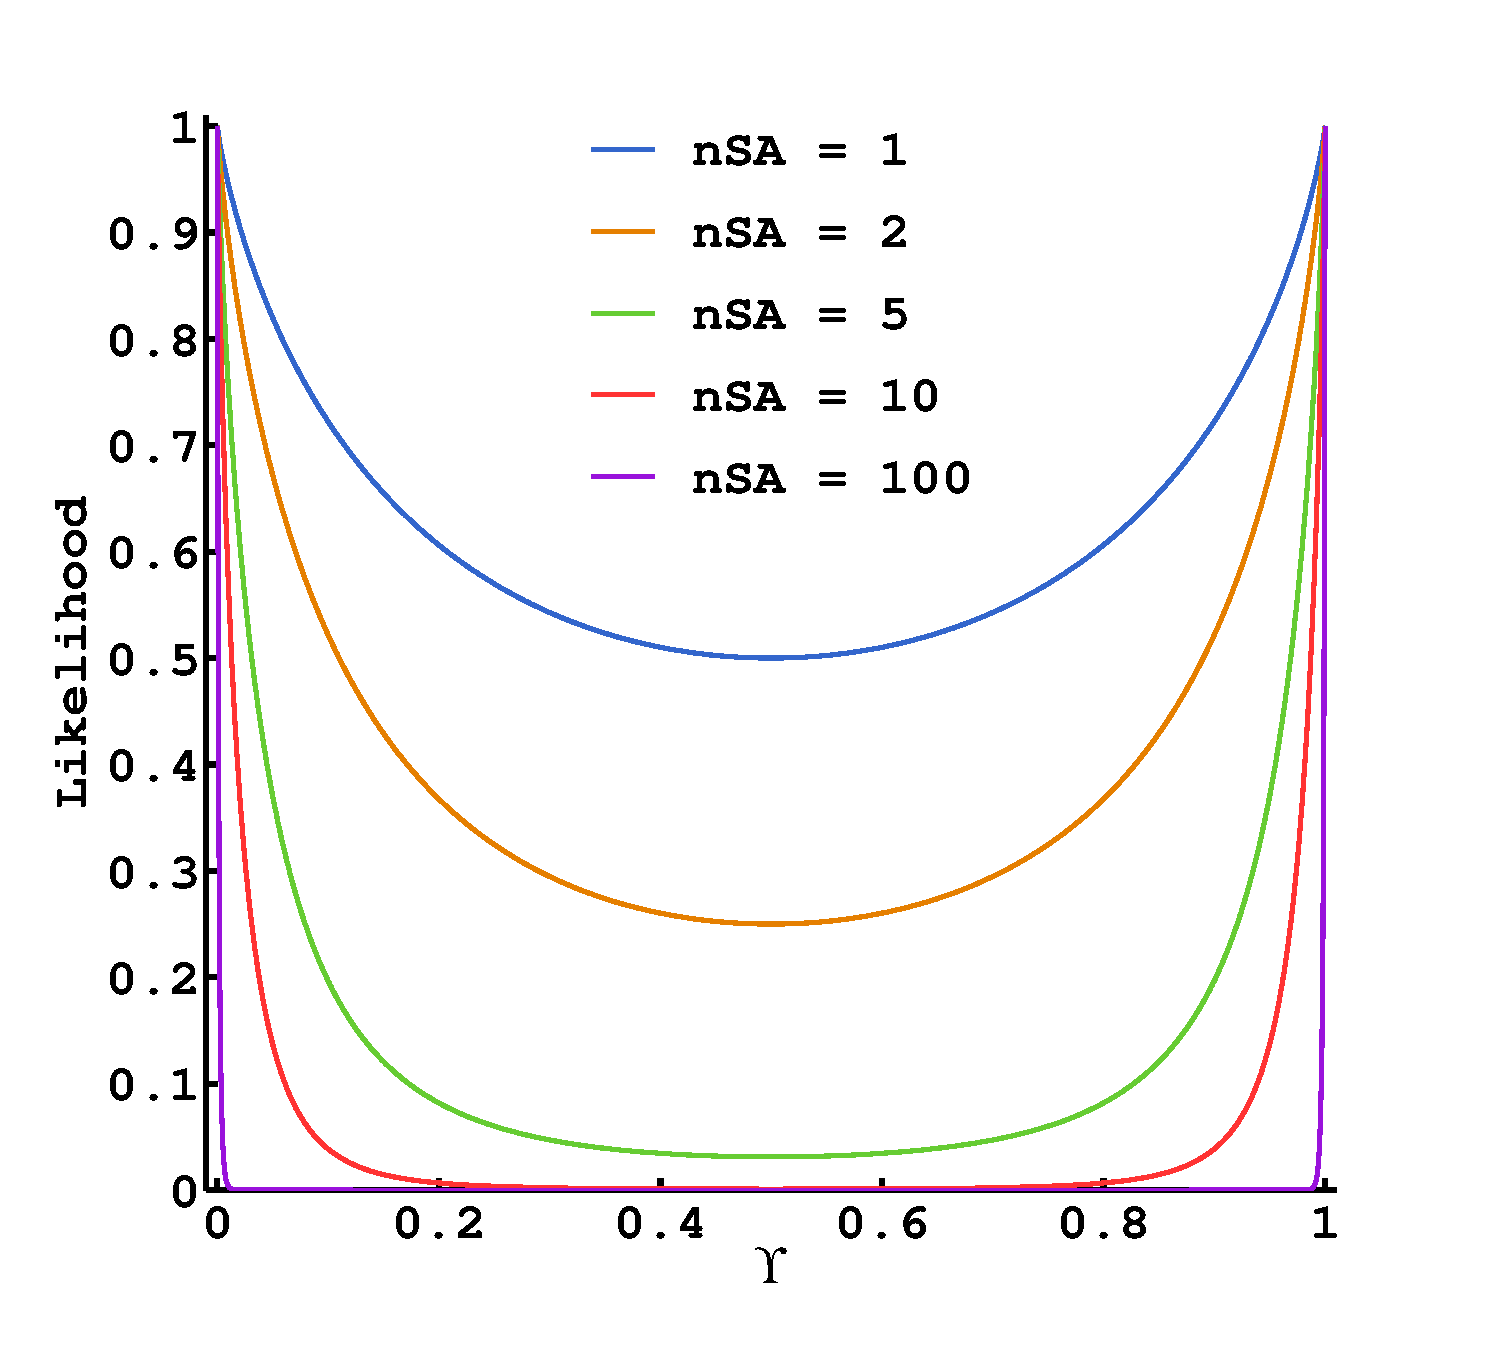
\includegraphics[width=\plotsize\columnwidth]{\imgpath/proof/likelihoodMany}
\caption{The likelihood function of Equation~\ref{eq:likelihoodproof} for $nSA =1,2,5,10,100$. The more we have collected evidence, the more the difference is sharp between task hypotheses.}
\label{fig:prooflikelihoodmany}
\end{figure}

This model allows understanding in more conceptual terms some properties of our algorithm. And in practice very few of the assumption considered are applicable in our experimental setups.

\visuopti{\newpage}

\subsubsection*{A simple scenario}

Finally, for illustration purpose, we present a world holding all our assumption properties, we named it the clock world (see Figure~\ref{fig:clockworld}). This world has 12 states, which we represent as the hours on a clock. The agent has two actions available: turning clockwise or counter-clockwise. The user wants the agent to reach one of 12 states. This world is the extension of the line word but where the line loops on itself.

\begin{figure}[!htbp]
\centering
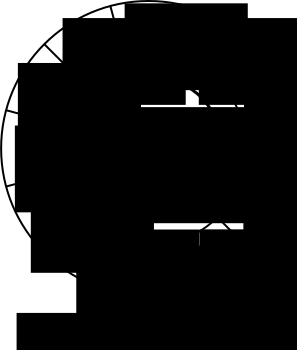
\includegraphics[width=0.3\columnwidth]{\visualspdf/proof/clockworld.pdf}
\caption{Illustration of the clock world. The agent has two actions available: turning clockwise or counter-clockwise. The user wants the agent to reach one of 12 states.}
\label{fig:clockworld}
\end{figure} 

\subsection{Why not using the entropy of the signal models?}

We continue here the discussion about the difference between the method detailed in chapter~\ref{chapter:lfui} of this thesis, where we differentiate between hypothesis by computing the probability that all signals are correctly classified, and the method presented in section~\ref{chapter:limitations:overlap}, where we consider only the signal models and differentiate between tasks by looking at the overlap of their Gaussian model associated to each class.

% In other words, we tried to evaluate the uncertainty of the signal model fitted for each task, and we selects the one that as lower uncertainty.

We can also apply a similar method than used in section~\ref{chapter:limitations:overlap} in our simple example. As we assumed that the user is coherent in his button presses, the task hypothesis whose associated button presses model is the less uncertain is the more likely to be the correct one. Given the history of interaction, we can model the button presses of the user as Bernoulli variables, which can take only two values ``correct'' or ``incorrect'', such as a coin-flipping problem. Following the previous development, we can compute the probability that the user will press the blue button to mean ``correct'', which is $\Upsilon_{\xi_t}$ (or $1-\Upsilon_{\xi_t}$ if the orange button is used for ``correct'').

The binary entropy function, denoted $H_{\mathrm b}(p)$, is the entropy of a Bernoulli process with probability of success p. It is a measure of uncertainty about the outcome of sampling from a Bernoulli process and can be computed as follows:

\begin{eqnarray}
H_{\mathrm b}(p) = -p\log_2(p) - (1-p)\log_2(1-p) 
\label{eq:likelihoodentropy}
\end{eqnarray}

The binary entropy function is shown in Figure~\ref{fig:prooflikelihoodentropy}. As one would expect the shape of the entropy function holds similar properties than our likelihood Equation~\ref{eq:likelihoodproof}.
    
\begin{figure}[!htbp]
\centering
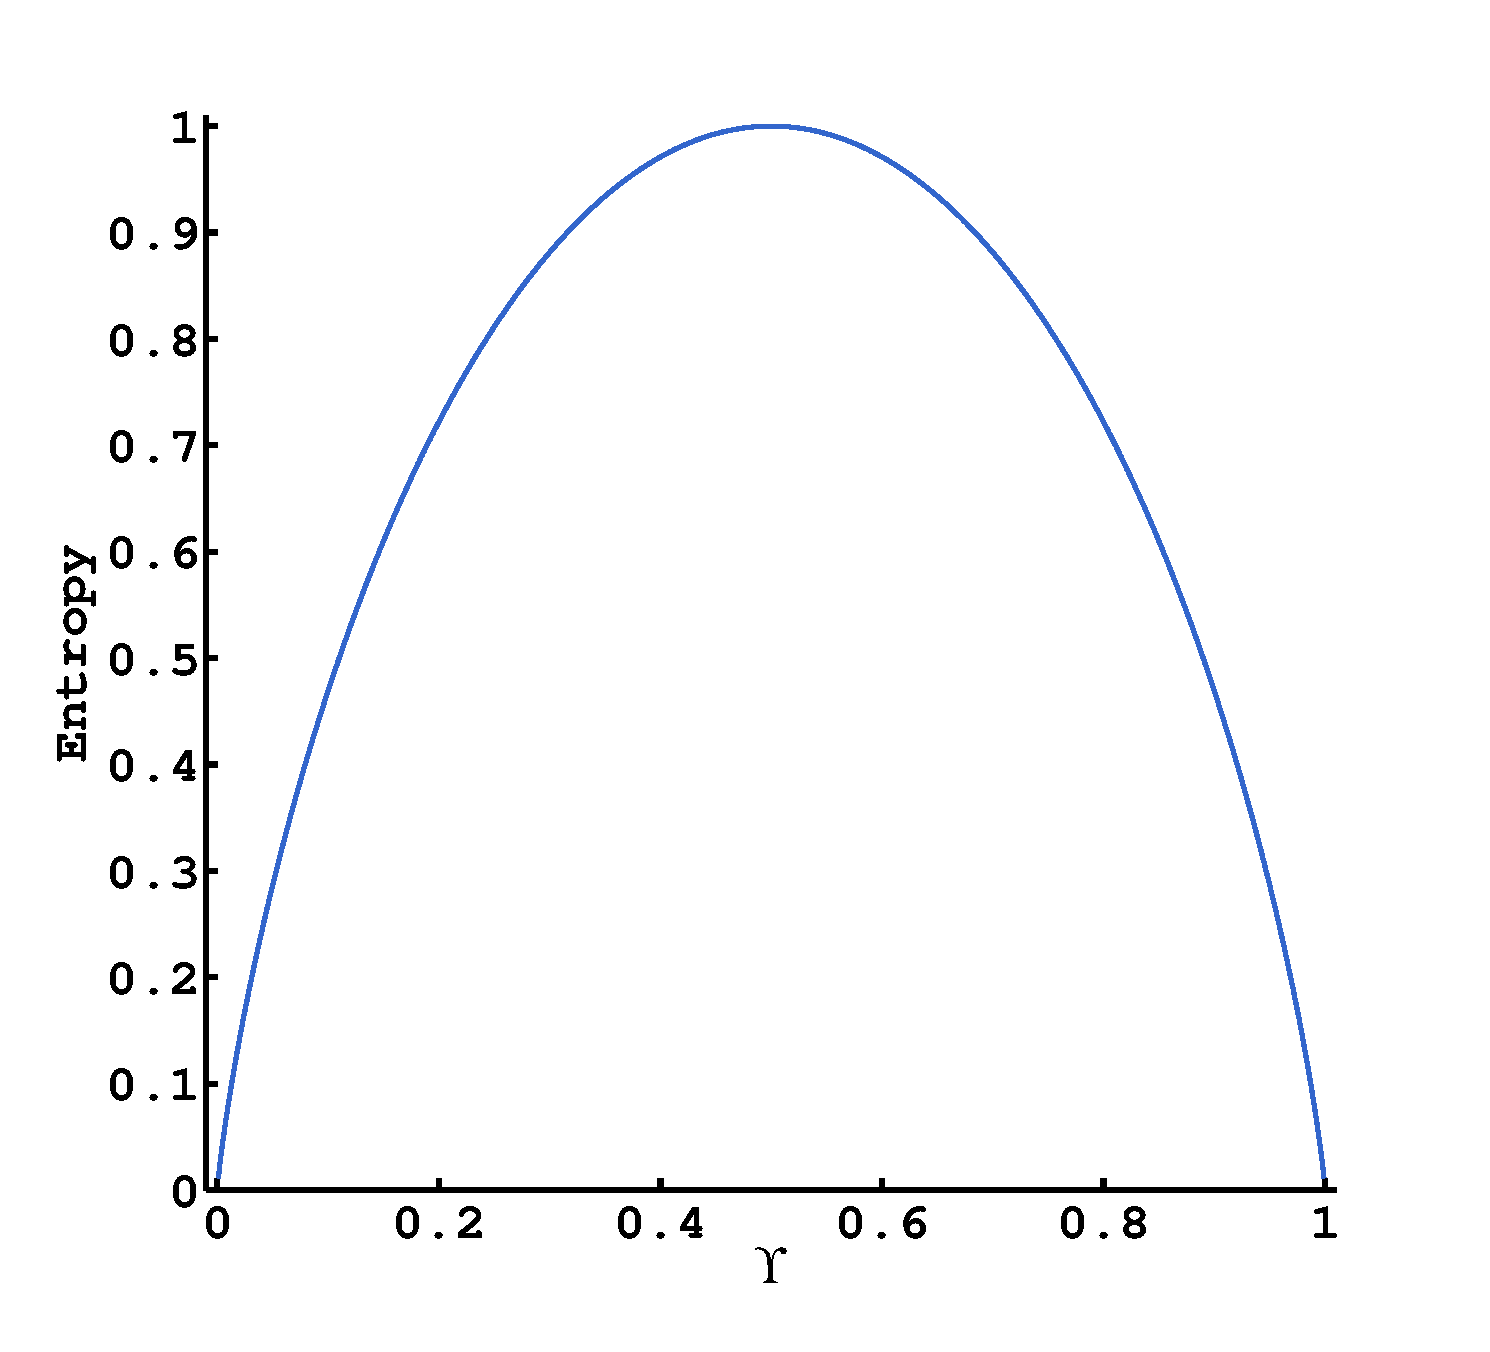
\includegraphics[width=\plotsize\columnwidth]{\imgpath/proof/entropy}
\caption{The binary entropy function.}
\label{fig:prooflikelihoodentropy}
\end{figure}

This method allows us to rank correctly our task hypothesis with respect to the uncertainty of their estimated models. However, this function will not ``sharpen'' when the agent visit more and more states. The only change will result in a better approximation of the Bernoulli process modeling the button presses.

Therefore, this method alone is not enough to estimate which task is the correct one, and we should also measure the uncertainty of this measure of uncertainty. To do so, we propose to use beta distribution, which is the conjugate prior probability distribution for the Bernoulli distributions. A beta distribution encodes a probability distribution over the parameter of the Bernoulli signal model given the amount of evidence available. By comparing between the beta distribution associated to each task, we could expect to find a suitable measure of task confidence. The interested readers may refer to \cite{montesano2012active} for a practical robotics example using this process.

\subsection{Discussion}

While it is always interesting and useful to formulate proof of algorithm, the restricted assumption used in this section makes it impossible to use this result in practical scenarios. But we note that our experimental results shows that our algorithm can work with fairly good performance on different scenarios using continuous signals as noisy as EEG signals.

% It may be useful to pursue in that direction by releasing some of the assumptions steps after steps. Starting with the assumption that all hypotheses have half of their state-action pair optimal and half non-optimal, and progressively accounting for some teaching mistakes. Reaching that level of proof would already offer some guarantees for simple scenarios using discrete state, discrete action, and symbolic signals, but under more realistic teaching conditions.

Nonetheless, it is important to pursue the theoretical analysis by progressively relaxing some assumptions. Sensible progresses can be achieved quickly, a first step is to consider a non-optimal user making uniform teaching mistakes and worlds with more realistic properties (e.g. with different ratios of optimal state-action pairs). Reaching that level of proof would already offer some guarantees for simple scenarios using discrete states, discrete actions, and symbolic signals, but under more realistic teaching conditions. The next step will be to consider non-symbolic signals, assuming they are sampled from latent distributions of known type.

